\chapter*{Annex}

\section{Electronics description}


The different pieces of electronics used in this experiment are described here.

\subsection{Amplifier}

Amplifiers are an electronic device which is used to increase the amplitude of a signal through modulation of output voltage or current. The ratio between the output amplitude and the input amplitude is called the \textit{Gain} ($G$). An example is shown in Figure \ref{fig:amplisin}

\begin{figure}[htbp]
\centering
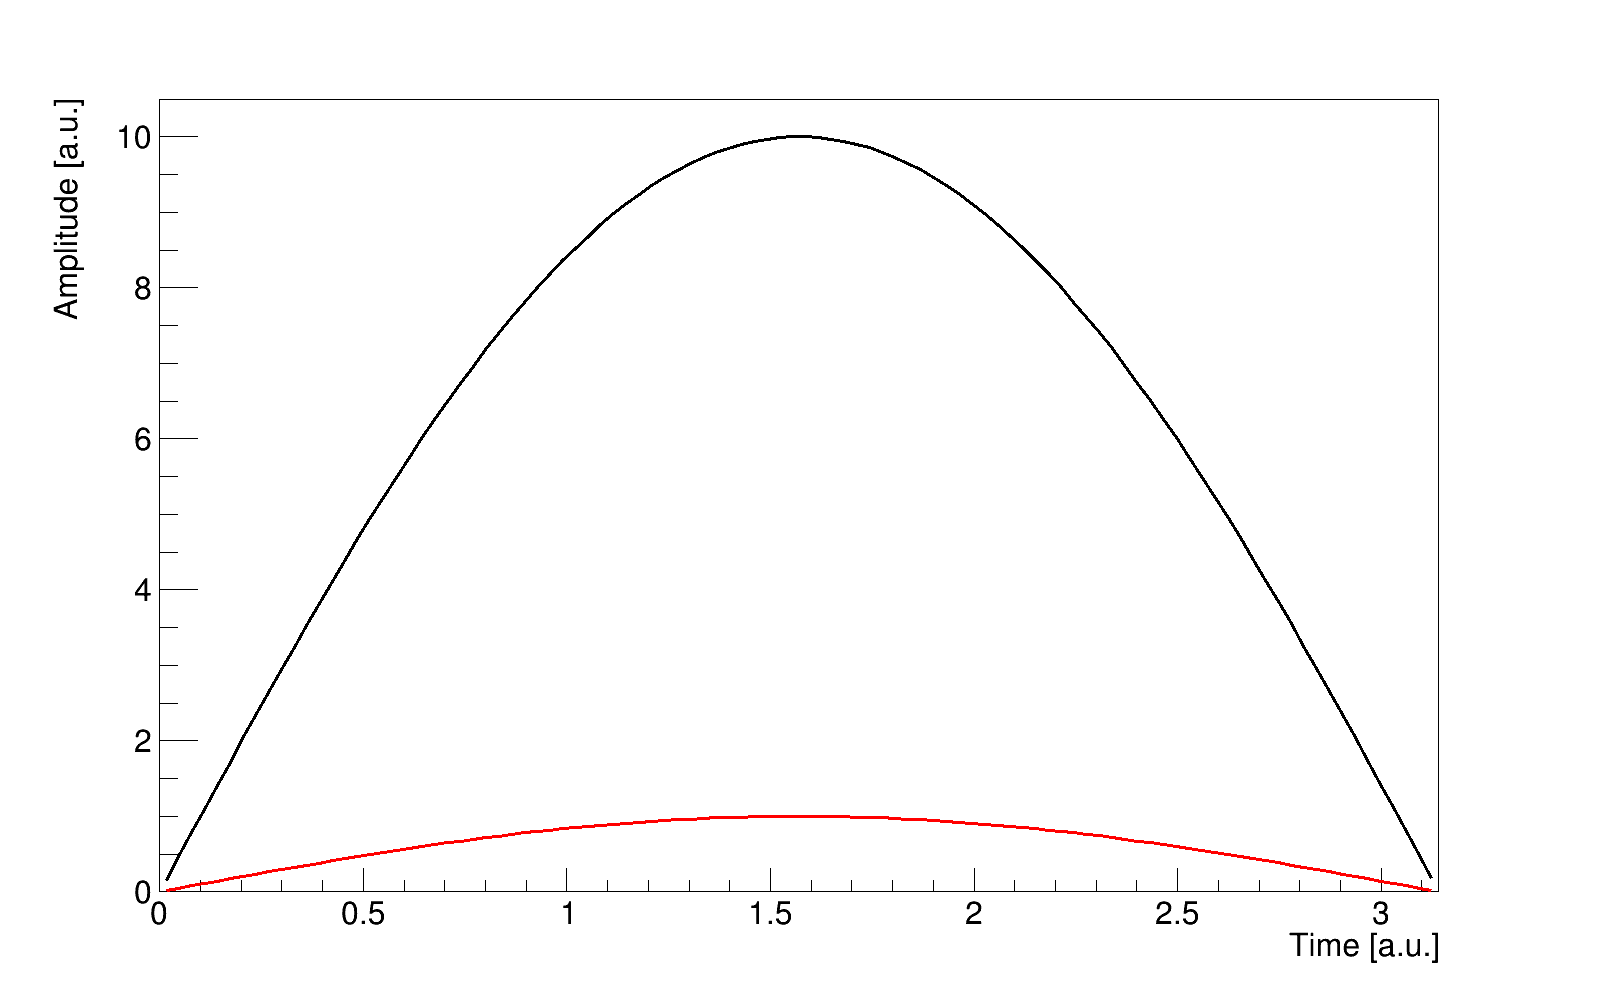
\includegraphics[width=0.7\linewidth]{./fig/amplisin.png}
\caption{Signal wave (red) and its ten-fold ($G=10$) amplified counterpart (black).}
\label{fig:amplisin}
\end{figure}

The experiment's amplifiers' gains can be tuned using a screwdriver on the holes left of the inputs.


\subsection{Discriminators}


Discriminators are an electronic Analog to Digital Converter (ADC). They produce a digital output when the signal fulfills certain conditions. If and when that is the case, a discriminator releases a single digital signal. Discriminators generally fall in one of two catergories: \textit{Leading Edge Discriminators} or \textit{Constant Fraction Discriminators} depending on which conditions they use to accept an analog signal:

\begin{itemize}

\item A leading edge discriminator only looks at the leading edge of signal, if the signal reaches the threshold level the logic pulse is emitted. This however can lead to \textit{walk}: time variance dependent on the size of the signal. This can increase difficulty in adjusting the timing information in the rest of the setup, and makes it impossible to obtain accurate timing information later. Thus, the constant fraction discriminator was created.

\item A constant fraction discriminator (CFD) works by looking at the entire signal and emits the logical pulse when the input signal reaches a certain fraction of its peak value. In this way a signal that has a wide time variance can be narrowed significantly using a leading edge discriminator.

\end{itemize}

The rate in the experiment being low and the timing not being critical at this stage of the circuit, the discriminators used here are of LE type.

\subsection{Monoflop unit}

Monoflops (shortened for \textit{Monostable Multivibrators}) are a sequential logic circuit that takes an input, two outputs and a clock unit (which may be seen as an extra input). The sequential part of the circuit (the clock) are continuous square function generators at a fixed frequency as shown in Figure 

\begin{figure}[htbp]
\centering
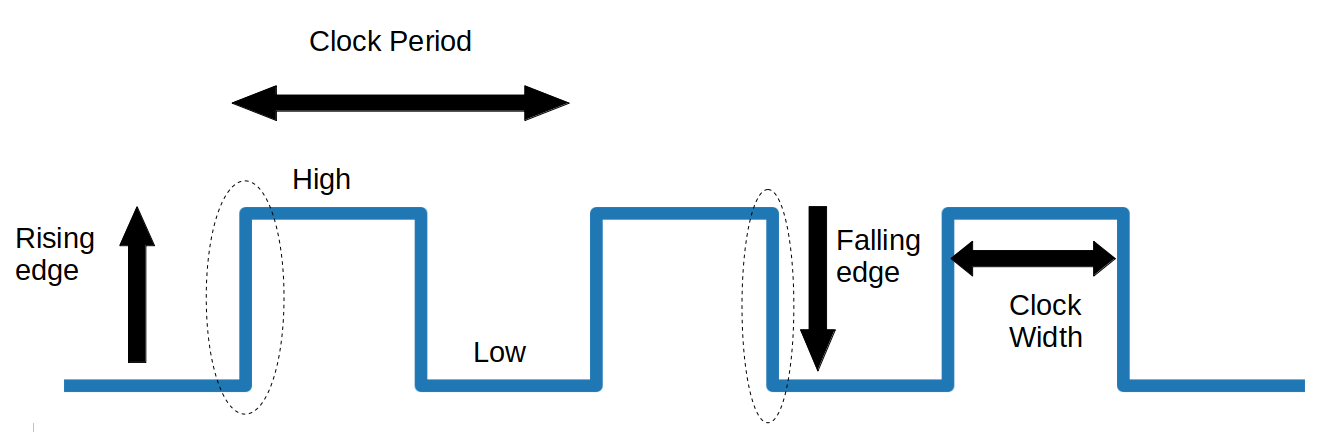
\includegraphics[width=0.7\linewidth]{./fig/rising.png}
\caption{Clock parameters.}
\label{fig:rising}
\end{figure}

Such sequential logic circuits using clock signals for synchronization depend on their frequency and therefore the clock pulse width to activate their switching action. Sequential circuits can also change their switching state using either the rising edge, falling edge, or both edges of the clock signal.

Monostable Multivibrators or “one-shot” pulse generators are generally used to convert short, sharp pulses into much wider ones for timing applications. Monosflops generate a single output pulse, either $1$ or $2$, when a suitable external trigger signal or start pulse T is applied.

This trigger pulse signal initiates a timing cycle which causes the output of the monostable to change state at the start of the timing cycle, ($t_1$). The ouput remains in this second state until the end of the timing period, ($t_2$) which is determined by the time constant of its timing capacitor, $CT$ and the resistor, $RT$.

The monostable multivibrator now stays in this second timing state until the end of the RC time constant and automatically “resets” or returns itself back to its original (stable) state.

In this experiment, the monoflop utilizes its clock to count over a set period of time, until it either received a second input (signaling a muon decay) or time runs out (no decay is seen/background).



